\section{Vectors}
  A \textbf{vector} indicates a quantity that has both magnitude and direction and is often represented by an arrow. The length of the arrow represents its magnitude and the direction represents the vector's direction. A vector is generally typed in boldface ($\mathbf{v}$) and written with an arrow above the letter ($\vec{v}$).\par
  Suppose a particle moves from $A$ to $B$, so its \textbf{displacement vector v} is $\vec{AB}$. The vector has \textbf{initial point} $A$ and \textbf{terminal point} $B$ and the vector is indicated by $\mathbf{v}=\vec{AB}$. Suppose another vector $\mathbf{u}$ has the same length and direction as $\mathbf{v}$ even though it is in a different position. We can say that $\mathbf{u}$ and $\mathbf{v}$ are \textbf{equivalent} (or \textbf{equal}) and we write $\mathbf{u} = \mathbf{v}$. The \textbf{zero vector}, denoted by \textbf{0}, has length 0. It is the only vector with no specific direction.
  \begin{definition}[\textbf{Definition of Vector Addition}]
    If \textbf{u} and \textbf{v} are vectors positioned so the initial point of \textbf{v} is at the terminal point of \textbf{u}, then the \textbf{sum} $\mathbf{u} + \mathbf{v}$ is the vector from the initial point of \textbf{u} to the terminal point of \textbf{v}.
  \end{definition}
  The definition of vector addition is sometimes called the \textbf{Triangle Law}. We can also use what we know about vectors to visualize the \textbf{Parallelogram Law}.
  \begin{center}
    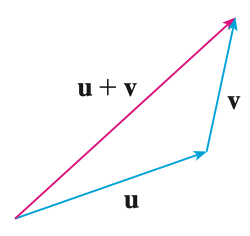
\includegraphics[width=.2\textwidth]{triangle_law.png}
    \hspace{45pt}
    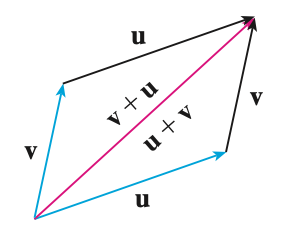
\includegraphics[width=.2\textwidth]{parallelogram_law.png}
  \end{center}
  \begin{definition}[\textbf{Definition of Scalar Multiplication}]
    If $c$ is a scalar and \textbf{v} is a vector, the the \textbf{scalar multiple} $c \mathbf{v}$ is the vector whose length is $|c|$ times the length of \textbf{v} and whose direction is the same as \textbf{v} if $c>0$ and is opposite if $c<0$. If $c=0$ or $\mathbf{v} = \mathbf{0}$, then $c\mathbf{v}=\mathbf{0}$.
  \end{definition}
  For instance, $2 \mathbf{v}$ is the same as $\mathbf{v} + \mathbf{v}$, which has the same direction as \textbf{v} but is twice as long.\par
  Two nonzero vectors are \textbf{parallel} if they are scaler multiples of one another. In particular, the vector $-\mathbf{v} = (-1)\mathbf{v}$ has the same length as \textbf{v} but points in the opposite direction and is called the \textbf{negative} of \textbf{v}.\\~\\
  The \textbf{difference} $\mathbf{u}-\mathbf{v}$ is $$ \mathbf{u}-\mathbf{v} = \mathbf{u}+ (-\mathbf{v})$$
  We can construct $\mathbf{u}-\mathbf{v}$ in two ways:
  \begin{enumerate}
    \item Draw the negative of \textbf{v}, $-\mathbf{v}$, and add it to \textbf{u} by the Parallelogram Law.
    \item $\mathbf{v}+(\mathbf{u}-\mathbf{v}=\mathbf{u}$, which also equals \textbf{u}, so we could construct $\mathbf{u}-\mathbf{v}$ by the Triangle Law.
  \end{enumerate}
  \begin{center}
    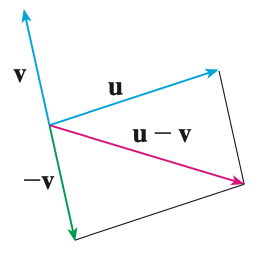
\includegraphics[width=.2\textwidth]{difference1.png}
    \hspace{45pt}
    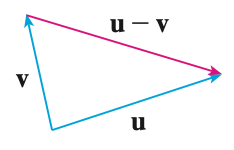
\includegraphics[width=.2\textwidth]{difference2.png}
  \end{center}
  \subsection*{Components}
    If we place the initial point of a vector \textbf{a} at the origin of a rectangular coordinate system, then the terminal point of \textbf{a} has coordinates of the form $(a_1,a_2)$ or $(a_1,a_2,a_3)$ depending on the dimensions of the coordinate system. These coordinates are called the \textbf{components} of \textbf{a}.
    $$\mathbf{a} = \langle a_1,a_2 \rangle \qquad \text{or} \qquad \mathbf{a} = \langle a_1,a_2,a_3 \rangle$$
    We use the notation $\langle a_1,a_2 \rangle$ that refers to a vector so we don't confuse it with the ordered pair $(a_1,a_2)$ that refers to a point in the plane.
    \begin{definition}
      Given the points $A(x_1,y_1,z_1)$ and $B(x_2,y_2,z_2)$, the vector \textbf{a} with representation $\vec{AB}$ is
      $$\mathbf{a}= \langle x_2-x_1,y_2-y_1,z_2-z_1 \rangle$$
    \end{definition}
    \begin{example}
      Find the vector represented by the directed line segment with initial point $A(2,-3,4)$ and $B(-2,1,1)$.
    \end{example}
    \begin{solution}
      The vector corresponding to $\vec{AB}$ is
      $$\mathbf{a}= \langle -2-2,\ 1-(-3),\ 1-4 \rangle = \langle -4,\ 4,\ -3 \rangle$$
    \end{solution}
    The \textbf{magnitude} or \textbf{length} of the vector \textbf{v} is the length of any of its representations and is denoted by the symbol $|v|$ or $\| v \|$. By using the distance formula to compute the length of a segment $OP$, we obtain the following formulas.
    \begin{definition}
      \hphantom{} \\
      The length of the two-dimensional vector $\mathbf{a} = \langle a_1,a_2 \rangle$ is
      $$ |\mathbf{a}| = \sqrt{a_{1}^{2} + a_{2}^{2}} $$
      The length of the three-dimensional vector $\mathbf{a} = \langle a_1,a_2,a_3 \rangle$ is
      $$ |\mathbf{a}| = \sqrt{a_{1}^{2} + a_{2}^{2} + a_{3}^{2}} $$
    \end{definition}
    \begin{definition}
      If $\mathbf{a} = \langle a_1,a_2 \rangle$ and $\mathbf{b} = \langle b_1,b_2 \rangle$, then
      \begin{align*}
        \mathbf{a+b} &= \langle a_1+b_1,a_2+b_2 \rangle \\
        \mathbf{a-b} &= \langle a_1-b_1,a_2-b_2 \rangle \\
        c \mathbf{a} &= \langle ca_1,ca_2 \rangle
        \intertext{Similarly, for three-dimensional vectors,}
        \langle a_1,a_2,a_3 \rangle + \langle b_1,b_2,b_3 \rangle &= \langle a_1+b_1,a_2+b_2,a_3+b_3 \rangle \\
        \langle a_1,a_2,a_3 \rangle - \langle b_1,b_2,b_3 \rangle &= \langle a_1-b_1,a_2-b_2,a_3-b_3 \rangle \\
        c\langle a_1,a_2,a_3 \rangle &= \langle ca_1,ca_2,ca_3 \rangle
      \end{align*}
    \end{definition}
    We denote $V_2$ as the set of all two-dimensional vectors and $V_3$ as the set of all three-dimensional vectors. More generally, we consider $V_n$ the set of all $n$-dimensional vectors. An $n$-dimensional vector is an ordered $n$-tuple:
    $$\mathbf{a} = \langle a_1,a_2,\ldots,a_n \rangle$$
    \begin{definition}[\textbf{Properties of Vectors}]
      If \textbf{a}, \textbf{b}, and \textbf{c} are vectors in $V_n$ and $c$ and $d$ are scalars, then
      \begin{enumerate}
        \item $\mathbf{a+b=b+a}$
        \item $\mathbf{a+(b+c) = (a+b)+c}$
        \item $\mathbf{a+0=a}$
        \item $\mathbf{a+(-a)=0}$
        \item $c \mathbf{(a+b)} = c \mathbf{a} + c \mathbf{b}$
        \item $(c+d)\mathbf{a} = c \mathbf{a} + d \mathbf{a}$
        \item $(cd)\mathbf{a}=c(d \mathbf{a})$
        \item $1\mathbf{a}=\mathbf{a}$
      \end{enumerate}
    \end{definition}
    Any vector in $V_3$ can be expressed in terms of the \textbf{standard basis vectors} $\mathbf{\hat{i}}$, $\mathbf{\hat{j}}$, and $\mathbf{\hat{k}}$. Such vectors are typically written with a hat. Let
    $$ \mathbf{\hat{i}}= \langle 1,0,0 \rangle \qquad \mathbf{\hat{j}}= \langle 0,1,0 \rangle \qquad \mathbf{\hat{k}}= \langle 0,0,1 \rangle$$
    Then $\mathbf{\hat{i}}$, $\mathbf{\hat{j}}$, and $\mathbf{\hat{k}}$ are vectors that have length 1 and point in the direction of the positive $x$-, $y$-, and $z$-axes. Similarly, in two dimensions we define $\mathbf{\hat{i}}= \langle 1,0 \rangle$ and $\mathbf{\hat{j}}= \langle 0,1 \rangle$.
    \begin{center}
      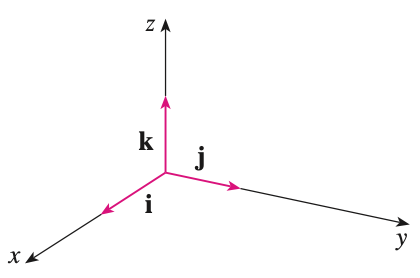
\includegraphics[width=.3\textwidth]{unit_vectors.png}
    \end{center}
    \begin{proof}\let\qed\relax
      We prove that these any vectors in $V_3$ can be in terms of $\mathbf{\hat{i}}$, $\mathbf{\hat{j}}$, and $\mathbf{\hat{k}}$.
      \\~\\
      If $\mathbf{a} = \langle a_1,a_2,a_3 \rangle$, then we write
      \begin{align*}
        \mathbf{a} &= \langle a_1,a_2,a_3 \rangle = \langle a_1,0,0 \rangle + \langle 0,a_2,0 \rangle + \langle 0,0,a_3 \rangle \\
        &= a_1\langle 1,0,0 \rangle + a_2\langle 0,1,0 \rangle + a_3\langle 0,0,1 \rangle \\
        \mathbf{a} &= a_1 \mathbf{\hat{i}} + a_2 \mathbf{\hat{j}} + a_3 \mathbf{\hat{k}}
        \intertext{Similarly, in two dimensions, we write}
        \mathbf{a} &= \langle a_1,a_2 \rangle  =a_1 \mathbf{\hat{i}} + a_2 \mathbf{\hat{j}}
      \end{align*}
    \end{proof}
    \begin{example}
      For instance,
      $$ \langle 1,-2,6 \rangle = \mathbf{\hat{i}} - 2\mathbf{\hat{j}} + 6\mathbf{\hat{k}} $$
    \end{example}
    A \textbf{unit vector} is a vector whose length is 1. For instance  $\mathbf{\hat{i}}$, $\mathbf{\hat{j}}$, and $\mathbf{\hat{k}}$ are all unit vectors.
    \begin{definition}
      In general, if $\mathbf{a \neq 0}$, then the unit vector that has the same direction as \textbf{a} is
      $$ \mathbf{u}= \frac{1}{|\mathbf{a}|}\mathbf{a} = \frac{\mathbf{a}}{|\mathbf{a}|} $$
    \end{definition}
    \begin{proof}\let\qed\relax
      Let $c=1/|\mathbf{a}|$. Then $\mathbf{u}=c \mathbf{a}$ and $c$ is a positive scalar, so \textbf{u} has the same direction as \textbf{a}. Also
      $$ |\mathbf{u}| = |c\mathbf{a}| = |c||\mathbf{a}| = \frac{1}{|\mathbf{a}|}\mathbf{a} = 1 $$
    \end{proof}
    \begin{example}
      Find the unit vector in the same direction of the vector $2\mathbf{\hat{i}} - \mathbf{\hat{j}} - 2\mathbf{\hat{k}}$.
    \end{example}
    \begin{solution}
      The given vector has length
      $$ |2\mathbf{\hat{i}} - \mathbf{\hat{j}} - 2\mathbf{\hat{k}}| = \sqrt{2^2 + (-1)^2 + (-2)^2} = \sqrt{9}=3$$
      We divide the vector by its length to find the unit vector with the same direction:
      $$ \tfrac{1}{3} (2\mathbf{\hat{i}} - \mathbf{\hat{j}} - 2\mathbf{\hat{k}}) = \tfrac{2}{3}\mathbf{\hat{i}} - \tfrac{1}{3}\mathbf{\hat{j}} - \tfrac{2}{3}\mathbf{\hat{k}} $$
    \end{solution}